\documentclass[12pt, a4paper]{article}

\usepackage[utf8]{inputenc}
\usepackage[T1]{fontenc}
\usepackage[spanish]{babel}
\usepackage{geometry}
\usepackage{graphicx}
\usepackage{hyperref}
\usepackage{listings}
\usepackage{xcolor}
\usepackage{float}
\usepackage{caption}
\usepackage{subcaption}
\usepackage{amsmath}
\usepackage{booktabs}
\usepackage{array}
\usepackage{parskip}
\usepackage{fancyhdr}

\geometry{a4paper, top=3cm, bottom=2.5cm, left=3cm, right=2.5cm}
\graphicspath{{../media/}}

\hypersetup{
    colorlinks=true,
    linkcolor=blue!60!black,
    urlcolor=blue!60!black,
    citecolor=green!50!black,
    pdftitle={Lane Keeping Control: Detección de Carriles y Seguimiento de Carril},
    pdfauthor={Agustín Mayor, Rafael Muñoz, José Francisco López},
}

\definecolor{codegreen}{rgb}{0,0.6,0}
\definecolor{codegray}{rgb}{0.5,0.5,0.5}
\definecolor{codepurple}{rgb}{0.58,0,0.82}
\definecolor{backcolour}{rgb}{0.97,0.97,0.97}
\lstdefinestyle{mystyle}{
    backgroundcolor=\color{backcolour},
    commentstyle=\color{codegreen}, keywordstyle=\color{blue},
    numberstyle=\tiny\color{codegray}, stringstyle=\color{codepurple},
    basicstyle=\ttfamily\footnotesize, breaklines=true,
    keepspaces=true, numbers=left, numbersep=5pt,
    showstringspaces=false, tabsize=2, frame=single,
    rulecolor=\color{gray!30}
}
\lstset{style=mystyle}

\pagestyle{fancy}
\fancyhf{}
\rhead{Control en Vehículos -- MIERA 2025/26}
\lhead{Detección y Seguimiento de Carril}
\cfoot{\thepage}

% ─────────────────────────────────────────────────────────────────────────────
\begin{document}
% ─────────────────────────────────────────────────────────────────────────────

\begin{titlepage}
    \centering
    \vspace*{2cm}
    {\large Universidad de Sevilla \par}
    {\large Máster en Ingeniería de Electrónica, Robótica y Automática (MIERA) \par}
    \vspace{1cm}
    {\large Control en Vehículos \par}
    \vspace{2cm}
    \hrule\vspace{0.5cm}
    {\Huge\bfseries Detección de Carriles y Control de Mantenimiento de Carril \par}
    \vspace{0.5cm}\hrule
    \vspace{2cm}
    {\large\itshape Grupo 1 \par}
    \vspace{1cm}
    \begin{tabular}{l}
        Agustín Mayor \\[4pt]
        Rafael Muñoz \\[4pt]
        José Francisco López
    \end{tabular}
    \vfill
    {\large Curso 2025--2026 \par}
\end{titlepage}

\tableofcontents
\newpage

\begin{abstract}
Este trabajo presenta el diseño e implementación de un sistema de \textit{Lane Keeping Assist} (LKA) para un vehículo autónomo simulado en \textit{CARLA Simulator} e integrado con \textit{ROS2 Humble} mediante contenedores Docker. El sistema consta de tres bloques principales: detección de líneas de carril mediante visión clásica con OpenCV y la transformada de Hough, diseño y sintonización de un controlador PID para mantener el vehículo centrado en el carril, y la integración de ambos módulos en un entorno de simulación realista donde se valida el funcionamiento completo. El código fuente, datasets e imágenes y vídeos demostrativos están disponibles en el repositorio público de GitHub: \url{https://github.com/JoseLopez36/Deteccion-Seguimiento-Carril}.
\end{abstract}

\newpage

% ═════════════════════════════════════════════════════════════════════════════
\section{Introducción}
% ═════════════════════════════════════════════════════════════════════════════

Los sistemas de asistencia a la conducción (ADAS) son hoy en día un componente fundamental tanto en la industria del automóvil como en la investigación en robótica móvil. Entre estos sistemas destaca el \textit{Lane Keeping Assist} (LKA), cuyo objetivo es mantener el vehículo centrado en su carril de forma autónoma, corrigiendo continuamente la dirección en función de la posición relativa del vehículo respecto a las marcas viales.

Este trabajo aborda el diseño e implementación de un sistema LKA completo, desde la adquisición de imagen hasta la actuación sobre los mandos del vehículo, validado en el simulador \textit{CARLA Simulator} mediante \textit{ROS2 Humble}. El flujo de funcionamiento del sistema es el siguiente:

\begin{enumerate}
    \item Adquisición de imágenes desde la cámara RGB frontal del vehículo simulado.
    \item Preprocesado de la imagen y detección de las líneas del carril mediante visión clásica.
    \item Cálculo del error lateral del vehículo respecto al centro del carril, expresado en metros a partir de los parámetros intrínsecos de la cámara.
    \item Generación de los comandos de aceleración/frenado y dirección mediante controladores PID, sintonizados previamente en MATLAB/Simulink.
    \item Publicación de los comandos de control al simulador CARLA.
\end{enumerate}

Todo el código fuente, datasets y material multimedia están disponibles en el repositorio público de GitHub del proyecto:
\begin{center}
    \url{https://github.com/JoseLopez36/Deteccion-Seguimiento-Carril}
\end{center}

\subsection*{Estructura de la memoria}

La memoria se organiza en tres bloques principales:

\begin{description}
    \item[Sección \ref{sec:carriles}: Detección de carriles.]
    Describe el pipeline de visión artificial empleado para detectar las marcas viales y calcular el error lateral del vehículo.
    \item[Sección \ref{sec:control}: Control de mantenimiento de carril.]
    Explica el modelado del vehículo y la sintonización del controlador PID en MATLAB/Simulink.
    \item[Sección \ref{sec:integracion}: Integración en simulación y resultados.]
    Desarrolla la arquitectura software completa en CARLA/ROS2, la infraestructura Docker, los nodos implementados y los resultados obtenidos.
\end{description}

% ═════════════════════════════════════════════════════════════════════════════
\section{Detección de carriles}
\label{sec:carriles}
% ═════════════════════════════════════════════════════════════════════════════

% TODO

% ═════════════════════════════════════════════════════════════════════════════
\section{Control de mantenimiento de carril}
\label{sec:control}
% ═════════════════════════════════════════════════════════════════════════════

% TODO

% ═════════════════════════════════════════════════════════════════════════════
\section{Integración en simulación y resultados}
\label{sec:integracion}
% ═════════════════════════════════════════════════════════════════════════════

Esta sección describe cómo los módulos de detección de carriles y control PID se integran en un sistema completo que opera en simulación en tiempo real. Se presentan el entorno de simulación empleado, la arquitectura software basada en ROS2, la infraestructura de contenedores Docker, los nodos que componen el sistema, la herramienta de monitorización y los resultados experimentales obtenidos.

% ─────────────────────────────────────────────────────────────────────────────
\subsection{Entorno de simulación: CARLA Simulator}
% ─────────────────────────────────────────────────────────────────────────────

Para el desarrollo y validación del sistema se ha empleado \textit{CARLA Simulator} (\textit{Car Learning to Act}), un simulador de conducción autónoma de código abierto basado en el motor gráfico \textit{Unreal Engine 4}. CARLA proporciona sensores virtuales de alta fidelidad —cámaras RGB, cámaras de segmentación semántica y medidores de velocidad— que permiten diseñar, depurar y validar algoritmos de percepción y control sin necesidad de un vehículo real.

El simulador se ejecuta en su versión \textit{0.9.15} dentro de un contenedor Docker con acceso a la GPU de la máquina anfitriona. Las principales características del entorno configurado son:

\begin{itemize}
    \item Mapa: Town04, escenario de carretera inter-urbana con marcas viales bien definidas.
    \item Vehículo (\textit{ego-vehicle}): modelo basado en el Tesla Model 3, controlado en lazo cerrado desde ROS2.
    \item Sensores disponibles:
    \begin{itemize}
        \item Cámara RGB frontal (\texttt{rgb\_front}): imagen principal usada para la detección de carriles.
        \item Cámara de segmentación semántica (\texttt{semantic\_segmentation\_front}): proporciona la máscara de \textit{ground truth} utilizada en la generación del dataset sintético.
        \item Medidor de velocidad (\texttt{speedometer}): velocidad actual del vehículo en m/s.
        \item Cámara exterior (\texttt{rgb\_view}): vista en tercera persona para supervisión visual.
    \end{itemize}
\end{itemize}

La Figura~\ref{fig:vistas_carla} muestra las dos perspectivas principales empleadas durante las sesiones de conducción autónoma.

\begin{figure}[H]
    \centering
    \begin{subfigure}[b]{0.48\textwidth}
        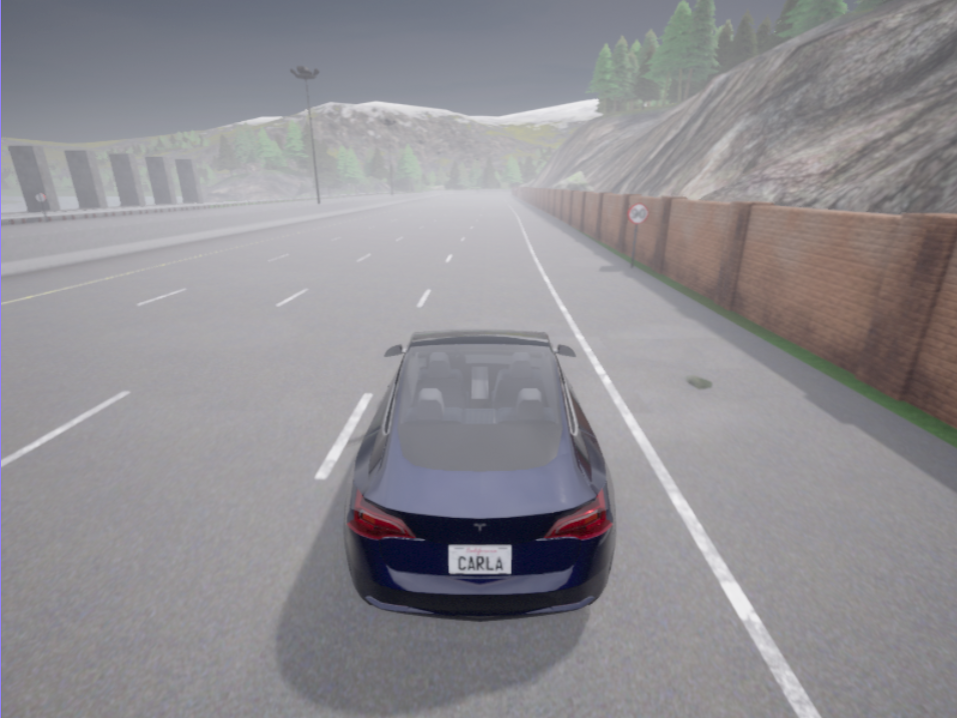
\includegraphics[width=\textwidth]{Vista_Externa.png}
        \caption{Vista exterior (tercera persona).}
    \end{subfigure}
    \hfill
    \begin{subfigure}[b]{0.48\textwidth}
        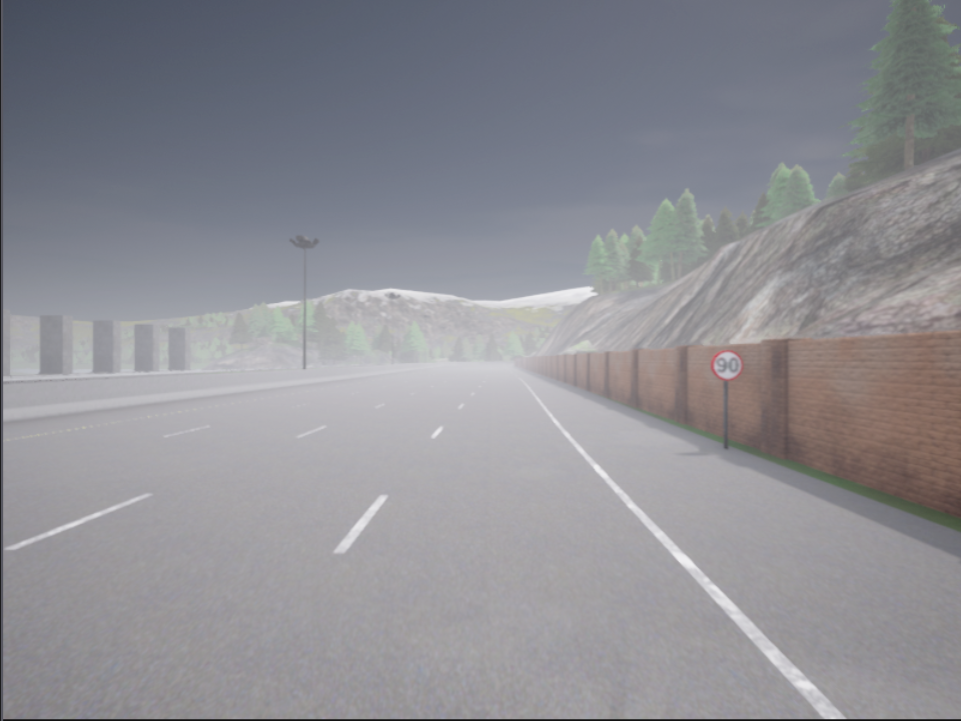
\includegraphics[width=\textwidth]{Vista_Camara_Frontal.png}
        \caption{Cámara frontal del vehículo.}
    \end{subfigure}
    \caption{Perspectivas en CARLA Simulator.}
    \label{fig:vistas_carla}
\end{figure}

% ─────────────────────────────────────────────────────────────────────────────
\subsection{Arquitectura del sistema}
% ─────────────────────────────────────────────────────────────────────────────

El sistema completo se organiza en tres capas que se comunican a través de una red Docker en modo \textit{host}:

\begin{enumerate}
    \item CARLA Simulator: simulador en su propio contenedor Docker con acceso a la GPU, que publica imágenes y telemetría como tópicos ROS2.
    \item CARLA-ROS2 Bridge: puente oficial (\texttt{carla\_ros\_bridge}) que traduce los datos de los sensores de CARLA en mensajes ROS2 estándar y convierte los comandos de control ROS2 en actuaciones sobre el vehículo simulado.
    \item Paquete de detección y control (\texttt{deteccion\_seguimiento\_carril}): paquete ROS2 propio que aloja los nodos de detección de carriles, control del vehículo y generación de anotaciones visuales.
\end{enumerate}

El flujo de datos es el siguiente: CARLA publica las imágenes de la cámara frontal en \texttt{/carla/ego\_vehicle/rgb\_front/image} y la velocidad en  \\ \texttt{/carla/ego\_vehicle/speedometer}. El \texttt{lane\_detection\_node} procesa cada \textit{frame} y publica el error lateral en metros en \texttt{/lane\_detection/lane\_error} y el estado completo del carril como JSON en \texttt{/lane\_detection/lane\_state}. El \texttt{vehicle\_control\_node} consume el error lateral y la velocidad para calcular y publicar los comandos de actuación en \texttt{/carla/ego\_vehicle/vehicle\_control\_cmd}. Por último, el \\ \texttt{annotation\_generator\_node} recoge el estado de todos los nodos y genera una capa de anotaciones visuales en \texttt{/foxglove/annotations}, que Foxglove Studio superpone sobre la imagen en tiempo real.

La Figura~\ref{fig:arquitectura} muestra el diagrama de bloques completo del sistema.

\begin{figure}[H]
    \centering
    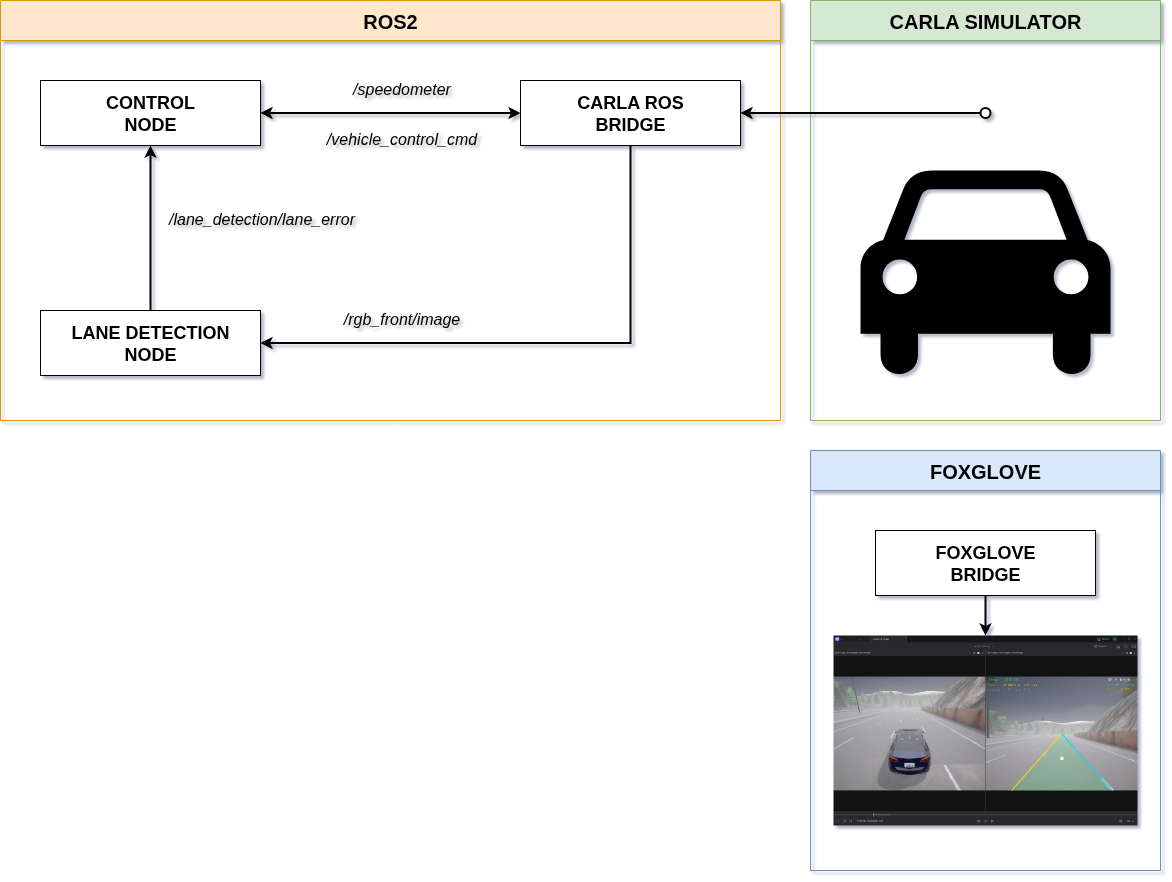
\includegraphics[width=0.95\textwidth]{diagram/Arquitectura.png}
    \caption{Diagrama de la arquitectura del sistema.}
    \label{fig:arquitectura}
\end{figure}

% ─────────────────────────────────────────────────────────────────────────────
\subsection{Infraestructura: Docker y contenedores}
% ─────────────────────────────────────────────────────────────────────────────

Todo el sistema se orquesta mediante \textbf{Docker Compose}, levantando los tres servicios con un único comando desde la raíz del repositorio:

\vspace{0.3cm}
\begin{lstlisting}[language=bash]
xhost +local:docker
docker compose -f tools/docker-compose.yaml up
\end{lstlisting}

La siguiente tabla describe cada uno de los servicios:

\begin{table}[H]
    \centering
    \label{tab:servicios_docker}
    \begin{tabular}{lll}
        \toprule
        \textbf{Servicio} & \textbf{Contenedor} & \textbf{Función} \\
        \midrule
        \texttt{ros\_bridge}  & \texttt{carla\_ros\_bridge}             & Bridge CARLA$\to$ROS2 \\
        \texttt{navegacion}   & \texttt{deteccion\_seguimiento\_carril} & Lanzamiento del paquete de ROS2 \\
        \texttt{foxglove}     & \texttt{foxglove\_bridge}               & WebSocket bridge para Foxglove Studio \\
        \bottomrule
    \end{tabular}
\end{table}

La imagen Docker base es \texttt{ros:humble-ros-base-jammy}, sobre la que se instalan ROS2 Humble Hawksbill, las librerías de visión artificial (\texttt{python3-opencv}, \texttt{ros-humble-cv-bridge}), las herramientas de visualización (\texttt{ros-humble-foxglove-bridge}, \texttt{ros-humble-foxglove-msgs}) y el cliente Python de CARLA~0.9.15 junto con el \texttt{carla-ros-bridge} compilado desde el código fuente.

El código fuente del paquete ROS2 se monta como volumen dentro del contenedor de navegación. Esto permite que cualquier cambio en el host quede disponible tras ejecutar \texttt{colcon build --symlink-install} sin necesidad de reconstruir la imagen Docker.

% ─────────────────────────────────────────────────────────────────────────────
\subsection{Nodos ROS2 del sistema}
% ─────────────────────────────────────────────────────────────────────────────

El paquete \texttt{deteccion\_seguimiento\_carril} implementa tres nodos ROS2 en Python que se lanzan de forma conjunta mediante \texttt{run.launch.py}, más un nodo adicional de recolecta de datos que se activa por separado.

\subsubsection{Nodo de detección de carriles (\texttt{lane\_detection\_node})}

Este nodo recibe cada \textit{frame} de de la cámara frontal y ejecuta el pipeline de visión clásica descrito en la Sección~\ref{sec:carriles}. A partir de las líneas detectadas calcula el error lateral del vehículo respecto al centro del carril: primero en píxeles (\texttt{offset\_px}) y luego en metros, dividiendo por la longitud focal $f_x$ extraída del mensaje \texttt{camera\_info}. Los resultados se publican en:
\begin{itemize}
    \item \texttt{/lane\_detection/lane\_error} (\texttt{std\_msgs/Float32}): error lateral en metros.
    \item \texttt{/lane\_detection/lane\_state} (\texttt{std\_msgs/String}): JSON con las coordenadas de las líneas izquierda y derecha, la zona de posición (\texttt{CENTER}/\texttt{LEFT}/\texttt{RIGHT}) y los flags de detección.
\end{itemize}

\subsubsection{Nodo de control del vehículo (\texttt{vehicle\_control\_node})}

Este nodo cierra el lazo de control: recibe el error lateral y la velocidad actual, y genera los comandos de actuación sobre el vehículo. Opera a 20~Hz e implementa dos controladores PID independientes.

\paragraph{PID de velocidad (control de crucero).}
Regula la velocidad del vehículo en torno a la referencia configurable \texttt{target\_speed}. El error de control es la diferencia entre la velocidad objetivo y la medida por el velocímetro. La salida del PID se mapea a los canales \textit{throttle} (acelerador) y \textit{brake} (freno) normalizados en $[0, 1]$:

\begin{align}
    e_v(t) &= v_{\text{ref}} - v_{\text{actual}} \notag \\
    u_v(t) &= K_{p,v}\,e_v + K_{i,v}\int e_v\,\mathrm{d}t \notag \\
    \text{throttle} &= \max(0,\,\min(1,\, u_v)), \quad
    \text{brake} = \max(0,\,\min(1,\,-u_v)) \notag
\end{align}

\paragraph{PID de dirección (mantenimiento de carril).}
Ajusta el ángulo del volante para mantener el vehículo centrado en el carril. El PID opera en radianes y su salida se normaliza por el ángulo físico máximo del volante ($\theta_{\max} = 0.6~\text{rad} \approx 34^\circ$) para obtener el valor de dirección normalizado de CARLA en $[-1,1]$. La convención de signo es: error positivo (vehículo desplazado a la derecha) produce una corrección hacia la izquierda (steer~$< 0$):

\begin{align}
    u_s(t) &= K_{p,s}\,e_s + K_{i,s}\int e_s\,\mathrm{d}t + K_{d,s}\,\dot{e}_s \notag \\
    \text{steer} &= \max\!\left(-1,\,\min\!\left(1,\,\frac{u_s}{\theta_{\max}}\right)\right) \notag
\end{align}

Ambos PIDs incorporan \textit{anti-windup} que limita el término integral al rango $[-10, 10]$. Los parámetros definitivos configurados en \texttt{params.yaml} se recogen en la Tabla~\ref{tab:pid}. Estos valores son el resultado de la sintonización en MATLAB/Simulink descrita en la Sección~\ref{sec:control}, trasladados directamente a la implementación en Python.

\subsubsection{Nodo generador de anotaciones (\texttt{annotation\_generator\_node})}

Este nodo actúa como capa de visualización del sistema. En cada \textit{frame} de la cámara frontal recoge el estado de los demás nodos y genera un mensaje \\ \texttt{foxglove\_msgs/ImageAnnotations} que Foxglove Studio superpone sobre la imagen en tiempo real. Las anotaciones incluyen:

\begin{itemize}
    \item Polígono de carril: región semitransparente en verde que cubre el área delimitada por las líneas izquierda y derecha detectadas.
    \item Líneas de carril: línea izquierda en amarillo y derecha en cian, con grosor de 5~px.
    \item Vector de desviación: segmento desde el centro geométrico de la imagen hasta el centro estimado del carril, en amarillo.
    \item HUD de telemetría: zona del carril (\texttt{CENTER}/\texttt{LEFT}/\texttt{RIGHT}), error lateral en metros y en píxeles, velocidad actual en km/h, y valores de \textit{throttle}, \textit{brake} y \textit{steer}.
\end{itemize}

La Figura~\ref{fig:interfaz} muestra la interfaz de Foxglove Studio durante una sesión de conducción.

\begin{figure}[H]
    \centering
    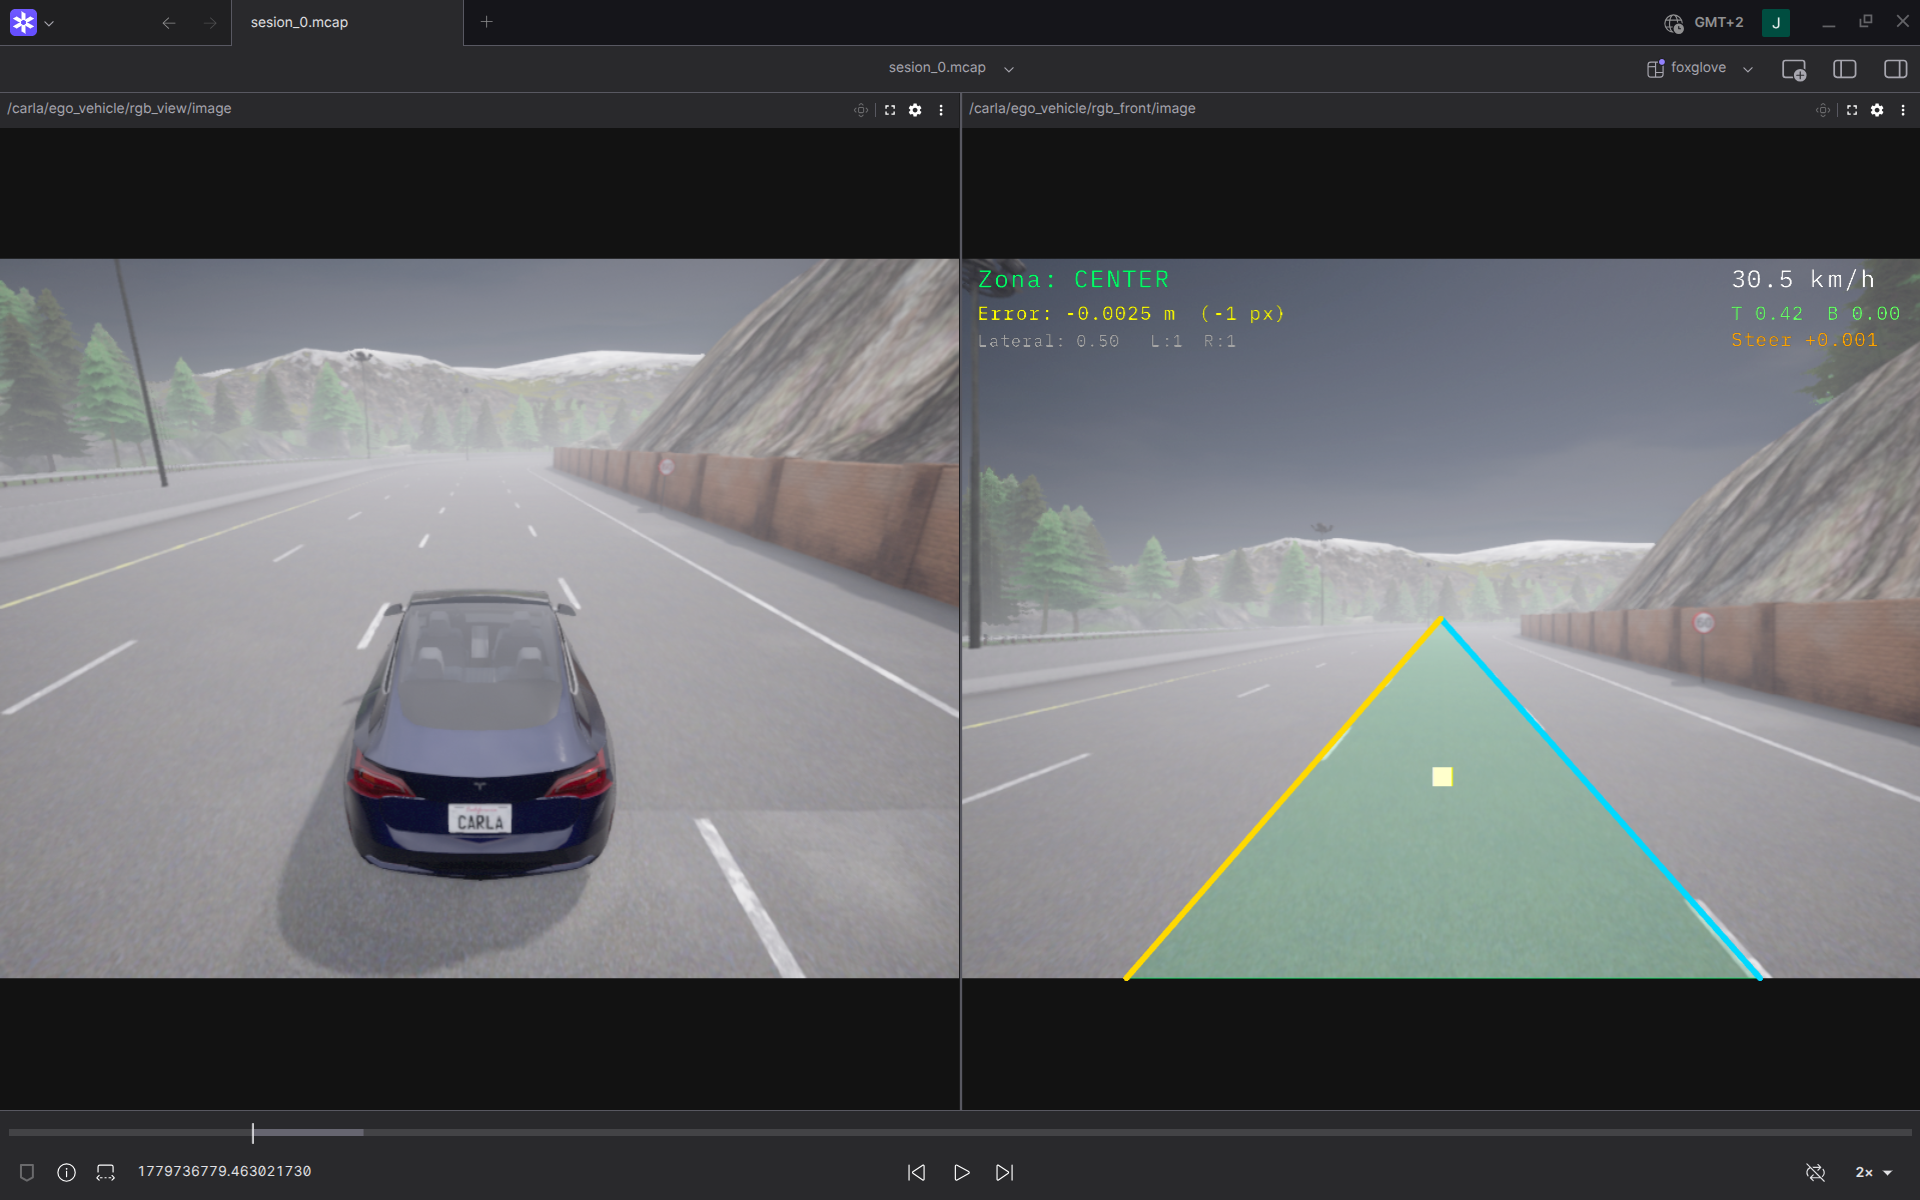
\includegraphics[width=\textwidth]{Interfaz.png}
    \caption{Interfaz de Foxglove Studio durante una sesión de conducción autónoma. A la izquierda, la vista exterior del vehículo; a la derecha, la cámara frontal con las anotaciones superpuestas: líneas del carril, polígono de área y HUD de telemetría.}
    \label{fig:interfaz}
\end{figure}

% ─────────────────────────────────────────────────────────────────────────────
\subsection{Generación de datasets sintéticos}
% ─────────────────────────────────────────────────────────────────────────────

Una de las ventajas de trabajar con un simulador como CARLA es la posibilidad de generar datos etiquetados de forma automática. La cámara de segmentación semántica asigna a cada píxel una etiqueta de clase con precisión perfecta, ofreciendo un \textit{ground truth} ideal para evaluar el detector de carriles sin ningún coste de anotación manual.

El nodo \texttt{lane\_dataset\_node} opera en modo conducción manual (sin el nodo de control) y captura imágenes a 5~Hz. Para cada instante capturado:
\begin{enumerate}
    \item Obtiene la máscara semántica del mismo instante de tiempo.
    \item Detecta los píxeles de marcas viales en la máscara y los proyecta sobre la imagen RGB.
    \item Almacena el par imagen~RGB / máscara binaria en \texttt{dataset/lanes/images/} y \texttt{dataset/lanes/masks/} respectivamente.
\end{enumerate}

La recolecta se lanza con:
\vspace{0.3cm}
\begin{lstlisting}[language=bash]
xhost +local:docker
docker compose -f tools/docker-compose-lane-dataset.yaml up
\end{lstlisting}

El repositorio incluye además la herramienta \texttt{tools/visualize\_lanes\_dataset.py} para revisar el dataset generado y \texttt{tools/make\_lane\_video.py} para producir un vídeo con el detector de carriles aplicado sobre las imágenes del dataset.

% ─────────────────────────────────────────────────────────────────────────────
\subsection{Resultados}
% ─────────────────────────────────────────────────────────────────────────────

Las pruebas de conducción autónoma se han realizado a dos velocidades de referencia: 18~km/h (5.0~m/s) y 30~km/h (8.33~m/s), modificando únicamente el parámetro \texttt{target\_speed} en \texttt{params.yaml}. En ambos casos el sistema es capaz de mantener el vehículo centrado en el carril de forma continuada sin intervención humana.

Los vídeos de las sesiones de conducción autónoma a 18~km/h y 30~km/h, así como un vídeo de demostración del detector de carriles sobre el dataset sintético, están disponibles en el repositorio público de GitHub:

\begin{center}
    \url{https://github.com/JoseLopez36/Deteccion-Seguimiento-Carril}
\end{center}

Los ficheros correspondientes son \texttt{media/Demo\_18\_kmh.mp4}, \texttt{media/Demo\_30\_kmh.mp4} y \texttt{media/Deteccion\_Carriles.mp4}.

% ═════════════════════════════════════════════════════════════════════════════
\section{Conclusiones}
% ═════════════════════════════════════════════════════════════════════════════

Este trabajo ha permitido implementar un sistema de \textit{Lane Keeping Assist} funcional de extremo a extremo, demostrando que la combinación de técnicas de visión clásica con un controlador PID en cascada y una arquitectura ROS2 modular constituye una solución eficaz y fácilmente reproducible para la conducción autónoma en simulación.

% TODO

\end{document}